\documentclass[12pt]{article}
\date{April 26, 2018}
\usepackage{pgf-pie}
\usepackage{pgfplots}
\usepackage{pgfplotstable}
\usetikzlibrary{patterns}
\usepackage[section]{placeins}
\usepackage[utf8]{inputenc}

\begin{document}


\clearpage{}
\section{Lorem ipsum dolor sit amët, \textbf{ consectetur } adipiscing elit.}

\label{sec:1}


\begin{figure}[h!]
    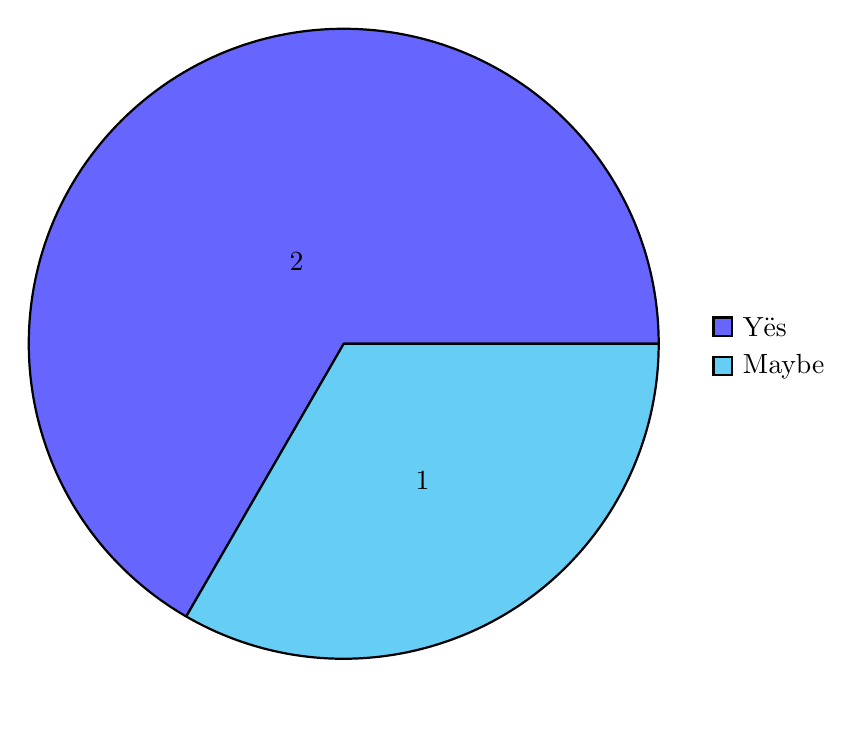
\begin{tikzpicture}
        \pie[radius=4,sum=auto,text=legend]{
            2/Yës,
            1/Maybe
        }
    \end{tikzpicture}
    \caption{\label{figure:q1-1}Repartition of answers for the question 'Lorem ipsum dolor sit amët, \textbf{ consectetur } adipiscing elit.'.}
\end{figure}



\clearpage{}
\section{Ipsum dolor sit amët, \textbf{ consectetur }  adipiscing elit.}

\label{sec:2}


\begin{figure}[h!]
    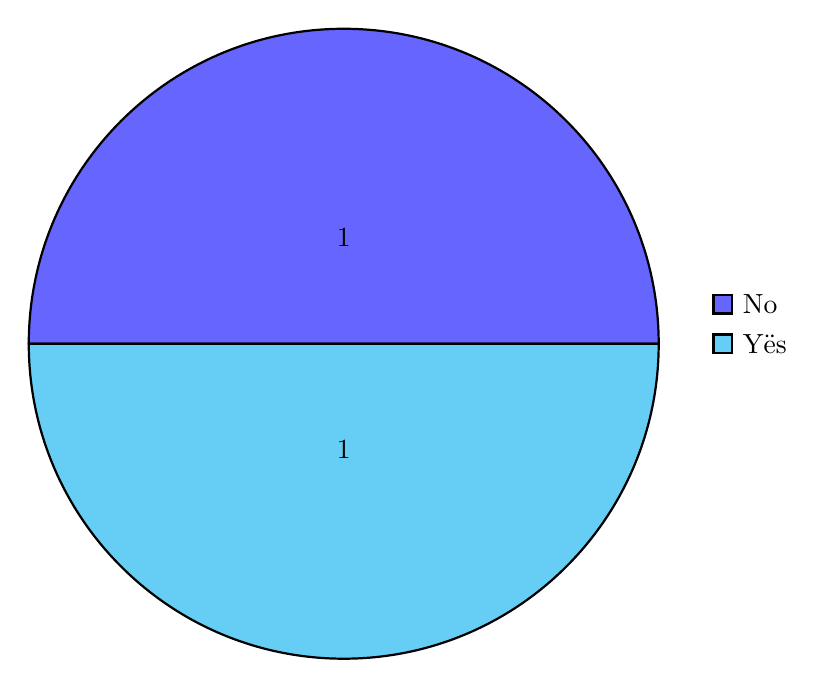
\begin{tikzpicture}
        \pie[radius=4,sum=auto,text=legend]{
            1/No,
            1/Yës
        }
    \end{tikzpicture}
    \caption{\label{figure:q2-1}Repartition of answers for the question 'Ipsum dolor sit amët, \textbf{ consectetur }  adipiscing elit.'.}
\end{figure}



\clearpage{}
\section{Dolor sit amët, \textbf{ consectetur}  adipiscing elit.}

\label{sec:3}


\begin{figure}[h!]
    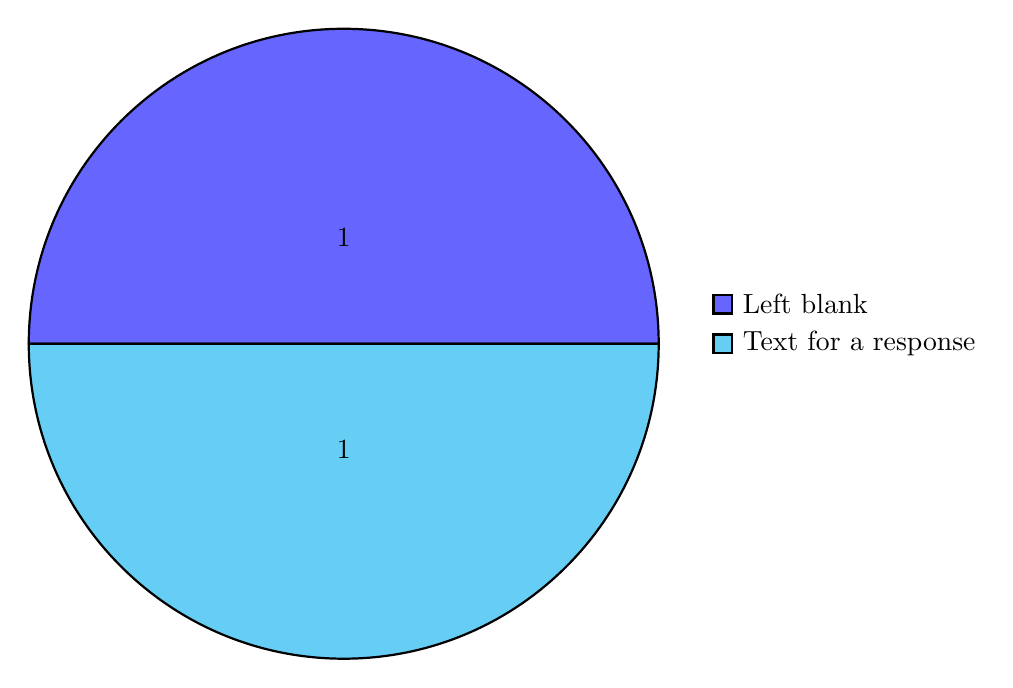
\begin{tikzpicture}
        \pie[radius=4,sum=auto,text=legend]{
            1/Left blank,
            1/Text for a response
        }
    \end{tikzpicture}
    \caption{\label{figure:q3-1}Repartition of answers for the question 'Dolor sit amët, \textbf{ consectetur}  adipiscing elit.'.}
\end{figure}



\clearpage{}
\section{Lorem ipsum dolor sit amët, consectetur\textbf{  adipiscing } elit.}

\label{sec:4}


\begin{figure}[h!]
    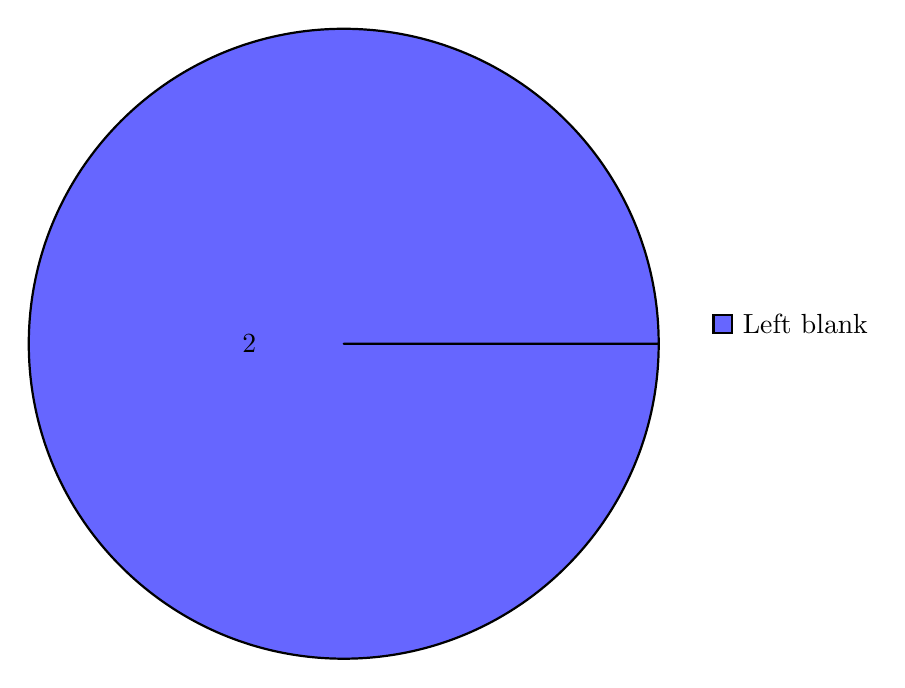
\begin{tikzpicture}
        \pie[radius=4,sum=auto,text=legend]{
            2/Left blank
        }
    \end{tikzpicture}
    \caption{\label{figure:q4-1}Repartition of answers for the question 'Lorem ipsum dolor sit amët, consectetur\textbf{  adipiscing } elit.'.}
\end{figure}



\clearpage{}
\section{Ipsum dolor sit amët, consectetur \textbf{ adipiscing } elit.}

\label{sec:5}


\begin{figure}[h!]
    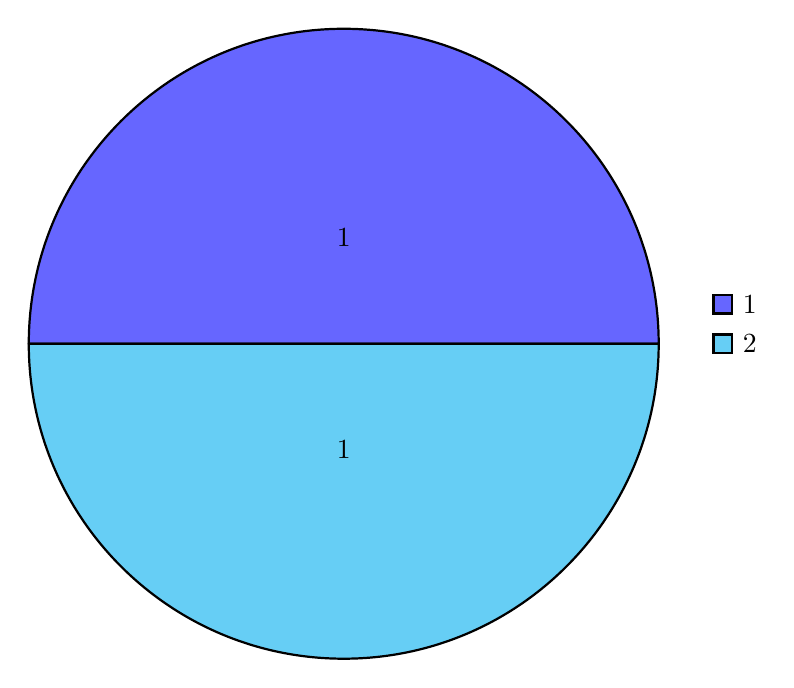
\begin{tikzpicture}
        \pie[radius=4,sum=auto,text=legend]{
            1/1,
            1/2
        }
    \end{tikzpicture}
    \caption{\label{figure:q5-1}Repartition of answers for the question 'Ipsum dolor sit amët, consectetur \textbf{ adipiscing } elit.'.}
\end{figure}



\clearpage{}
\section{Dolor sit amët, consectetur\textbf{  adipiscing}  elit.}

\label{sec:6}


\begin{figure}[h!]
    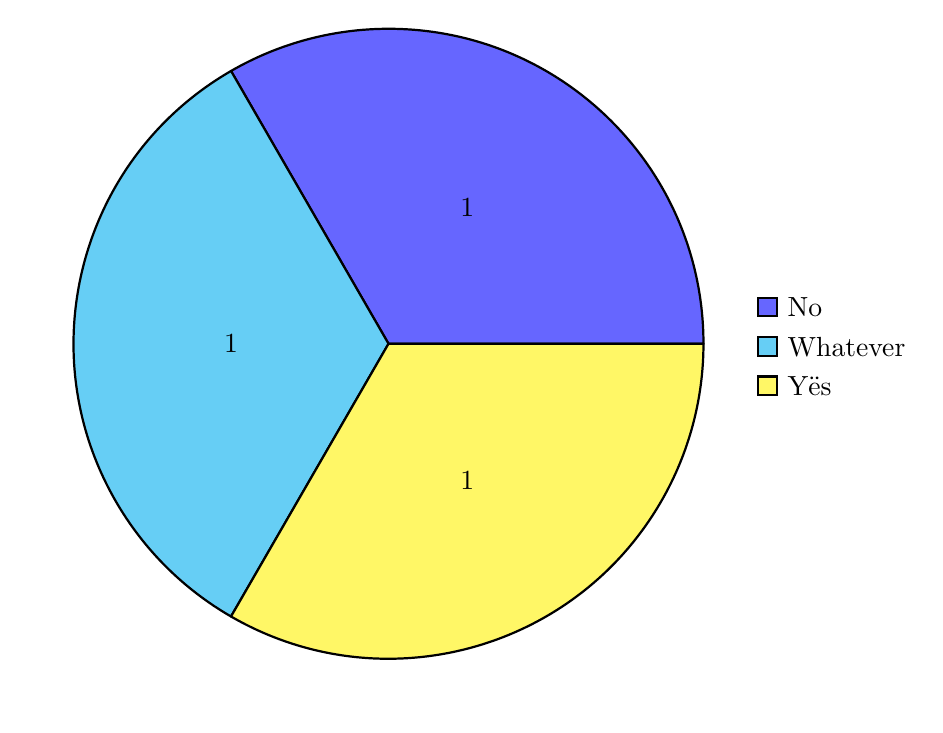
\begin{tikzpicture}
        \pie[radius=4,sum=auto,text=legend]{
            1/No,
            1/Whatever,
            1/Yës
        }
    \end{tikzpicture}
    \caption{\label{figure:q6-1}Repartition of answers for the question 'Dolor sit amët, consectetur\textbf{  adipiscing}  elit.'.}
\end{figure}



\end{document}
